
\begin{figure}[t]
\vspace{-2.0mm}
  \centering
  \begin{subfigure}[b]{0.65\textwidth}
    % \includegraphics[width=\textwidth]{tex/images/overview.pdf}
    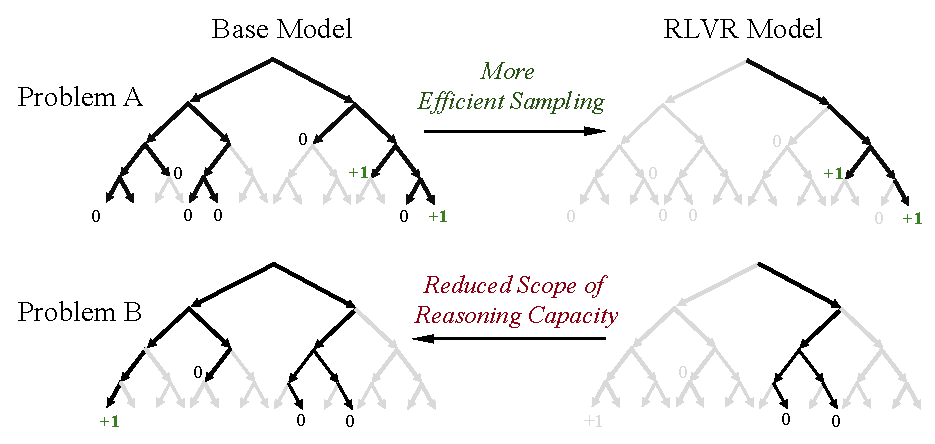
\includegraphics[width=\textwidth]{tex/images/overview2.pdf}
  \end{subfigure}
  \hfill
    \begin{subfigure}[b]{0.3\textwidth}
    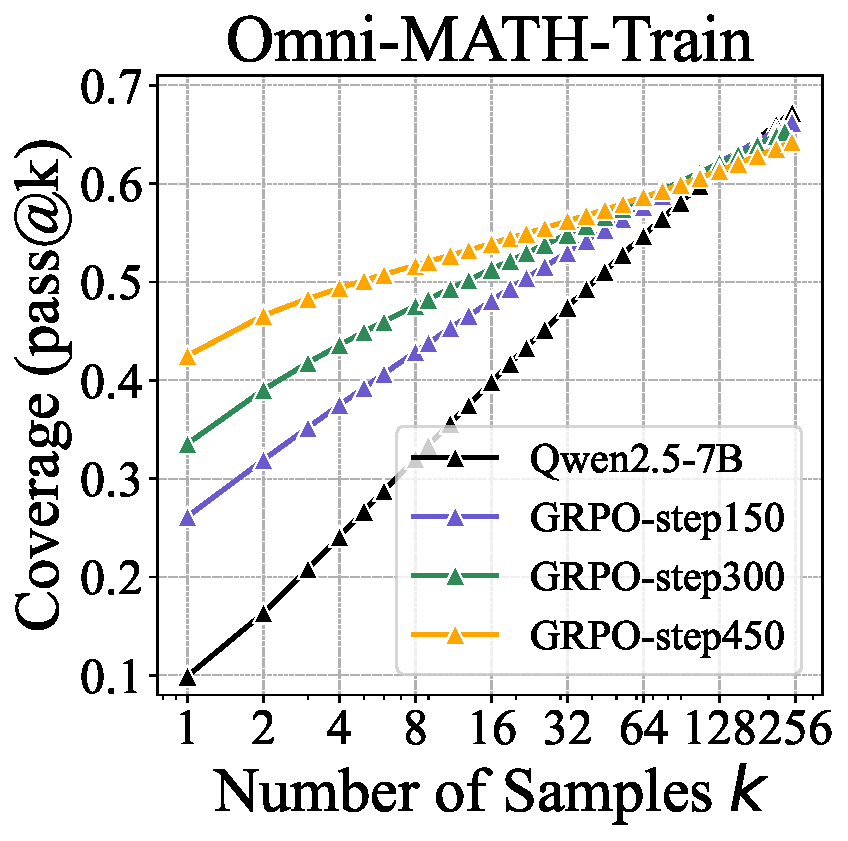
\includegraphics[width=\textwidth]{tex/images/qwen25_7b_base_step_coverage_v2_only_train.pdf}
  \end{subfigure}
\captionsetup{font={footnotesize}}
\caption{
\textbf{(Left)} The effect of current RLVR on LLM's reasoning ability.
Search trees are generated by repeated sampling from the base and RLVR-trained models for a given problem.
\textcolor{darkgrey}{Grey} indicates paths that are unlikely to be sampled by the model, while \textbf{black} indicates paths that are likely to be sampled. \textcolor{darkgreen}{Green} indicates correct paths, which has positive rewards.
Our key finding is that all reasoning paths in the RLVR model are already present in the base model.
For certain problems like Problem A, RLVR training biases the distribution toward rewarded paths, improving sampling efficiency.
However, this comes at the cost of reduced scope of reasoning capacity: For other problems like Problem B, 
% the scope of reasoning capacity of 
the base model contains the correct path, whereas that of the RLVR model does not.
\textbf{(Right)}
As RLVR training progresses, the average performance (\ie, pass@1) improves, but the coverage of solvable problems (\ie, pass@256) decreases, indicating a reduction in LLM's reasoning boundary.
}
\label{fig:overview}
\vspace{-5mm}
\end{figure}

\vspace{-2.0mm}
\section{Introduction}
\vspace{-0.5mm}


% 1. Introduce the scuccess of RLVR and the insight behind RL
The development of reasoning-centric large language models (LLMs), such as OpenAI-o1~\cite{jaech2024openaio1}, DeepSeek-R1~\cite{guo2025deepseek-r1}, and Kimi-1.5~\cite{team2025kimi}, has significantly advanced the frontier of LLM capabilities, particularly in solving complex logical tasks involving mathematics and programming. 
In contrast to traditional instruction-tuned approaches that rely on human-curated annotations~\cite{achiam2023gpt4, grattafiori2024llama3}, the key driver behind this leap forward is large-scale \textit{Reinforcement Learning with Verifiable Rewards} (RLVR)~\cite{lambert2024tulu3,guo2025deepseek-r1}. RLVR starts with a pretrained base model or one fine-tuned on long chains of thought (CoT) data, optimizing it via reinforcement learning based on simple, automatically computable rewards. These rewards are determined by whether the model's output matches a ground-truth solution in mathematics or passes unit tests in code, thus enabling scalability without human labeling.
This framework has gained significant attention due to its simplicity and practical effectiveness. 
In traditional RL settings such as game playing (\eg, Atari, Go), agents often autonomously discover new strategies and surpass even human-level performance through self-improvement~\cite{mnih2015dqn, silver2017alphagozero}. Inspired by this success, it is widely believed that RLVR similarly enables LLMs to autonomously develop novel reasoning patterns, including enumeration, self-reflection, and iterative refinement, surpassing the capabilities of their base models~\cite{guo2025deepseek-r1}. Consequently, RLVR has been considered a promising path toward continuously self-evolving LLMs, potentially bringing us closer to more powerful intelligence~\cite{guo2025deepseek-r1}.

% 2. Raise the question and propose research methodology
% However, despite these empirical successes, a critical question remains largely unexplored: \textbf{\textit{Does current RLVR genuinely introduce novel reasoning capabilities to LLMs beyond those already present in the base model?}}
However, despite its empirical success, the underlying effectiveness of current RLVR remains underexamined. This raises a fundamental question: \textit{\textbf{Does current RLVR genuinely enable LLMs to acquire novel reasoning abilities--similar to how traditional RL discovers new strategies through exploration--or does it simply utilize reasoning patterns already in the base model?}}

To rigorously answer this question, we must first assess the reasoning capability boundaries of both base and RLVR-trained models. Traditional evaluation metrics rely on average score from greedy decoding or nucleus sampling~\cite{holtzman2019topp}, which reflects average-case behavior. However, these metrics risk underestimating the true potential of a model, especially if it fails on difficult problems after limited attempts, despite being capable of solving them with more sampling.
To overcome this limitation, we adopt the pass@\textit{k} metric~\cite{brown2024monkey}, where a problem is considered solved if any of the $k$ sampled outputs is correct. By allowing multiple attempts, pass@\textit{k} reveals whether a model has the potential to solve a problem. 
The average pass@\textit{k} across a dataset thus reflects the proportion of problems a model can potentially solve within $k$ trials, offering a more robust view of its reasoning boundary. 
This provides a rigorous test on whether the RLVR training yields fundamentally transcending capacity, enabling the model to solve problems that the base model cannot.

Using the pass@\textit{k} metric, we conduct extensive experiments across various benchmarks, 
% spanning mathematics, code generation, and visual reasoning, 
covering multiple LLM families, model sizes, and RLVR algorithms to compare base models with their RLVR-trained counterparts.
% We find several perhaps surprising discoveries that may alter the conventional understanding of reasoning models and RLVR training, as follows:
We uncover several surprising findings that offer a more comprehensive assessment of the effectiveness of current RLVR training and reveal the gap between existing RLVR methods and the ideal goals of RL-discovering genuinely new reasoning strategies:

% \textbf{$\bullet$ RLVR-trained models perform worse than base models in pass@$k$ at large $k$ values.}
%  Although RLVR models consistently outperform their base models in small $k$, it is highly surprising that base models consistently surpass RLVR models across all benchmarks and LLM families as $k$ increases. This means that the base model without any RLVR training can already generate the correct answers to problems that were previously considered only solvable for RL-trained models by aggressively sampling different approaches. We manually check the CoTs of these correct answers and find most of problems has \textit{at least one} CoT to be correct. This suggests that RL training does \emph{not} improve, but even downgrade, LLMs' potential scope of reasoning capability. 

\textbf{$\bullet$ Current RLVR models often exhibit narrower reasoning coverage than their base models.}
In pass@$k$ curves, although RLVR models outperform their base models at small $k$, it is surprising that base models consistently surpass RLVR models across all benchmarks and LLM families as $k$ increases. 
This suggests that current RLVR training does \emph{not} expand, and even reduce the scope of reasoning over solvable problems.
Manual inspection of model responses shows that, for most problems, the base model can produce \textit{at least one} correct CoT, implying that it can already generate correct reasoning paths for problems that were previously considered only solvable for RLVR models. 


 % \textbf{$\bullet$ RLVR boosts sampling efficiency at the cost of reducing the scope of reasoning capacity.} 
%  To further investigate this phenomenon, we conduct perplexity analysis. Our findings show that reasoning paths generated by RLVR-trained models already exist within the base models' output distribution with considerable probability density, indicating that these reasoning patterns and CoTs are not totally strange and unachievable for base models. 
%  As RL is designed for, RLVR training contributes to reasoning by biasing the model toward rewarded reasoning paths, thereby increasing the likelihood of sampling correct reasoning paths.
%  However, this efficiency gain also comes at a cost: RL training reduces the model's exploration capacity, resulting in smaller coverage of solvable problems at large $k$ (see ~\cref{fig:overview} right), suggesting its reduced scope of reasoning capacity.
% This challenges the common belief that RLVR elicits transcending reasoning ability. 
% Instead, the reasoning capacity boundary of RLVR-trained models may be bounded by the capabilities of base model.
% The effect of RLVR on LLM's reasoning ability is illustrated in~\cref{fig:overview} left.

\textbf{$\bullet$ Reasoning paths generated by current RLVR model already exist in its base model.}
To further investigate this phenomenon, we analyze the accuracy distribution.
The results show that although RLVR improves average performance (\ie, pass@1) by sampling more efficiently on problems already solvable by the base model, it does not enable the model to solve new problems.
Further perplexity analysis reveals that the reasoning paths produced by RLVR models already exist within the output distribution of the base model. 
These findings indicate that RLVR does not introduce fundamentally new reasoning capabilities and that the reasoning capacity of current RLVR models remains bounded by that of its base model.
This effect of RLVR is illustrated in~\cref{fig:overview} (left).


\textbf{$\bullet$ Current RLVR algorithms perform similarly and remain far from optimal.}  
Treating the base model as an upper bound, we define the \textit{sampling efficiency gap} ($\Delta_{\text{SE}}$), shown in~\cref{fig:algo_and_step} (top), as the difference between an RL model's pass@1 and the base model's pass@$k$ (with $k=256$ as a proxy for upper-bound performance). This metric quantifies how closely an RL algorithm approaches the optimal bound.  
Across all algorithms (e.g., PPO, GRPO, Reinforce++), $\Delta_{\text{SE}}$ shows only minor variation yet remains consistently large, suggesting that current RLVR methods, while improving sampling efficiency, are still far from optimal.


\textbf{$\bullet$ RLVR and distillation are fundamentally different.}
While RLVR improves reasoning scores by more efficiently sampling high-reward outputs, it does not elicit new reasoning capabilities and remains constrained within the base model's capacity. 
In contrast, distillation can transfer new reasoning patterns from a stronger teacher to the student. As a result, distilled models often demonstrate an expanded reasoning scope beyond that of the base model.

In conclusion, our findings show that current RLVR methods, while improving sampling efficiency, rarely elicit novel reasoning beyond the base model. 
This highlights a gap between existing RLVR methods and the goals of reinforcement learning, underscoring the need for improved RL paradigms such as better exploration, continual data scaling, fine-grained process signal, and multi-turn agent interaction.
